\chapter{异常}

\section{异常}

\subsection{异常(Exception)}

异常就是程序在运行过程中出现的非正常的情况。异常本身是一个类,产生异常就是创建异常对象并抛出一个异常对象。Java处理异常的方法是中断处理。\\

C++异常处理涉及到三个关键字:

\begin{enumerate}
	\item throw:当问题出现时,程序会抛出一个异常。
	\item try:放置可能抛出异常的代码。
	\item catch:捕获并处理异常。
\end{enumerate}

\begin{figure}[H]
	\centering
	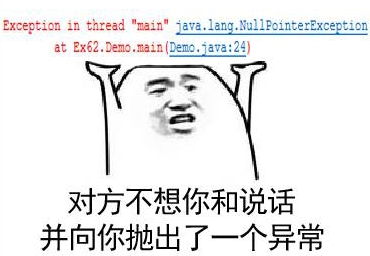
\includegraphics{img/C5/5-1/1.png}
\end{figure}

\mybox{除以0}

\begin{lstlisting}[language=C++]
#include <iostream>

using namespace std;

int divide(int num1, int num2) {
    if(num2 == 0) {
        throw "division by zero";
    }
    return num1 / num2;
}

int main() {
    try {
        int result = divide(5, 0);
        cout << result << endl;
    } catch(const char *msg) {
        cerr << msg << endl;
    }

    return 0;
}
\end{lstlisting}

\begin{tcolorbox}
	\mybox{运行结果}
	\begin{verbatim}
division by zero
	\end{verbatim}
\end{tcolorbox}

普通的异常会导致程序无法完成编译,这样的异常被称为非运行时异常(non-runtime exception),但是由于异常是发生在编译时期的,因此常常称为编译时异常。在运行中如果遇到了异常,会导致程序执行的强制停止,这样的异常被称为运行时异常。

\newpage

\section{异常类}

C++提供了一系列标准的异常,定义在<exception>中。

\begin{table}[H]
	\centering
	\setlength{\tabcolsep}{5mm}{
		\begin{tabular}{|c|l|}
			\hline
			\textbf{异常}          & \textbf{描述}         \\
			\hline
			std::exception         & 所有标准C++异常的父类 \\
			\hline
			std::bad\_alloc        & 通过new抛出           \\
			\hline
			std::bad\_cast         & 通过dynamic\_cast抛出 \\
			\hline
			std::bad\_exception    & 处理无法预期的异常    \\
			\hline
			std::bad\_typeid       & 通过typeid抛出        \\
			\hline
			std::logic\_error      & 逻辑错误              \\
			\hline
			std::domain\_error     & 使用了无效的定义域    \\
			\hline
			std::invalid\_argument & 使用了无效的参数      \\
			\hline
			std::length\_error     & 创建过长的std::string \\
			\hline
			std::out\_of\_range    & 访问定义外的元素      \\
			\hline
			std::runtime\_error    & 运行时错误            \\
			\hline
			std::overflow\_error   & 发生上溢              \\
			\hline
			std::underflow\_error  & 发生下溢              \\
			\hline
			std::range\_error      & 存储超出范围的值      \\
			\hline
		\end{tabular}
	}
	\caption{异常类}
\end{table}

what()是异常类提供的一个公共方法,它已被所有子异常类重载。\\

\mybox{bad\_alloc}

\begin{lstlisting}[language=C++]
#include <iostream>
#include <exception>

using namespace std;

int main() {
    try {
        char *p = new char[0xfffffffff];
        delete p;
    } catch(bad_alloc &e) {
        cerr << e.what() << endl;
    }
    return 0;
}
\end{lstlisting}

\begin{tcolorbox}
	\mybox{运行结果}
	\begin{verbatim}
std::bad_alloc
	\end{verbatim}
\end{tcolorbox}

\newpage

\section{自定义异常}

\subsection{自定义异常}

系统中提供了很多的异常类型,但是异常类型提供地再多,也无法满足所有的需求。当需要的异常类型系统没有提供的时候,此时就需要自定义异常了。通过继承和重载exception类可以定义新的异常。\\

\mybox{自定义异常}

\begin{lstlisting}[language=C++]
#include <iostream>
#include <string>
#include <exception>

using namespace std;

class AgeException : public exception {
public:
    AgeException(string msg) : msg(msg) {}

    virtual const char* what() const noexcept override {
        return msg.c_str();
    }

private:
    string msg;
};

int main() {
    try {
        int age;
        cout << "Enter age: ";
        cin >> age;
        if(age < 0 || age > 130) {
            throw AgeException("invalid age");
        }
    } catch(AgeException& e) {
        cout << e.what() << endl;
    }

    return 0;
}
\end{lstlisting}

\begin{tcolorbox}
	\mybox{运行结果}
	\begin{verbatim}
Enter age: -1
invalid age
	\end{verbatim}
\end{tcolorbox}

\newpage